\section{Reservoir Computing}

%\begin{frame}{Reservoir computing in a nutshell...}
%	\begin{itemize}
%		\item Reservoir Computing (RC) is a \emph{artificial neural network} scheme that allows real-time data processing
%		\item Reservoir maps the input to a higher dimensional space
%		\item The \emph{neurons} are connected in a way that leads to a chaotic behaviour of the reservoir (achieved by using randomness, breaking symmetries,...)
%		\item The input is fed into the reservoir and disturbs the intrinsic dynamics of the neurons
%		\item Output is found by adequately combining the activation level of the neurons
%		\item This scheme is so general that it can be implemented on physical systems
%		\item It reaches state-of-the-art time series prediction algorithms
%	\end{itemize}
%\end{frame}

\begin{frame}{Reservoir Computing (RC) in a nutshell...}
	\begin{itemize}
		\item Artificial Neural Network
		\item Real-time data processing scheme
		\item Can be implemented in physical systems
		\item State of the art performances in time series prediction
	\end{itemize}
\end{frame}

\begin{frame}{Mathematical model of a RC}
	\begin{columns}[T] % align columns
	\begin{column}{.48\textwidth}
	
		Discrete time dynamics of a neuron \cite{JaegerH.2001Tesa}:
		
		\begin{multline}
			x_i (t+1) = f_{NL} \biggl( W^{ij}~x_j(t)\\ + W^{ij}_{\text{in}}~u_j(t)+W^{ij}_{\text{fb}}~y_j(t) \biggl)
		\end{multline}
		
		Discrete time output of the reservoir:
		
		\begin{equation}
			y_i(t) = W^{ij}_{\text{out}} ~x_j(t)
		\end{equation}
	
	\end{column}%
	\hfill%
	\begin{column}{.48\textwidth}
	
	\begin{figure}
		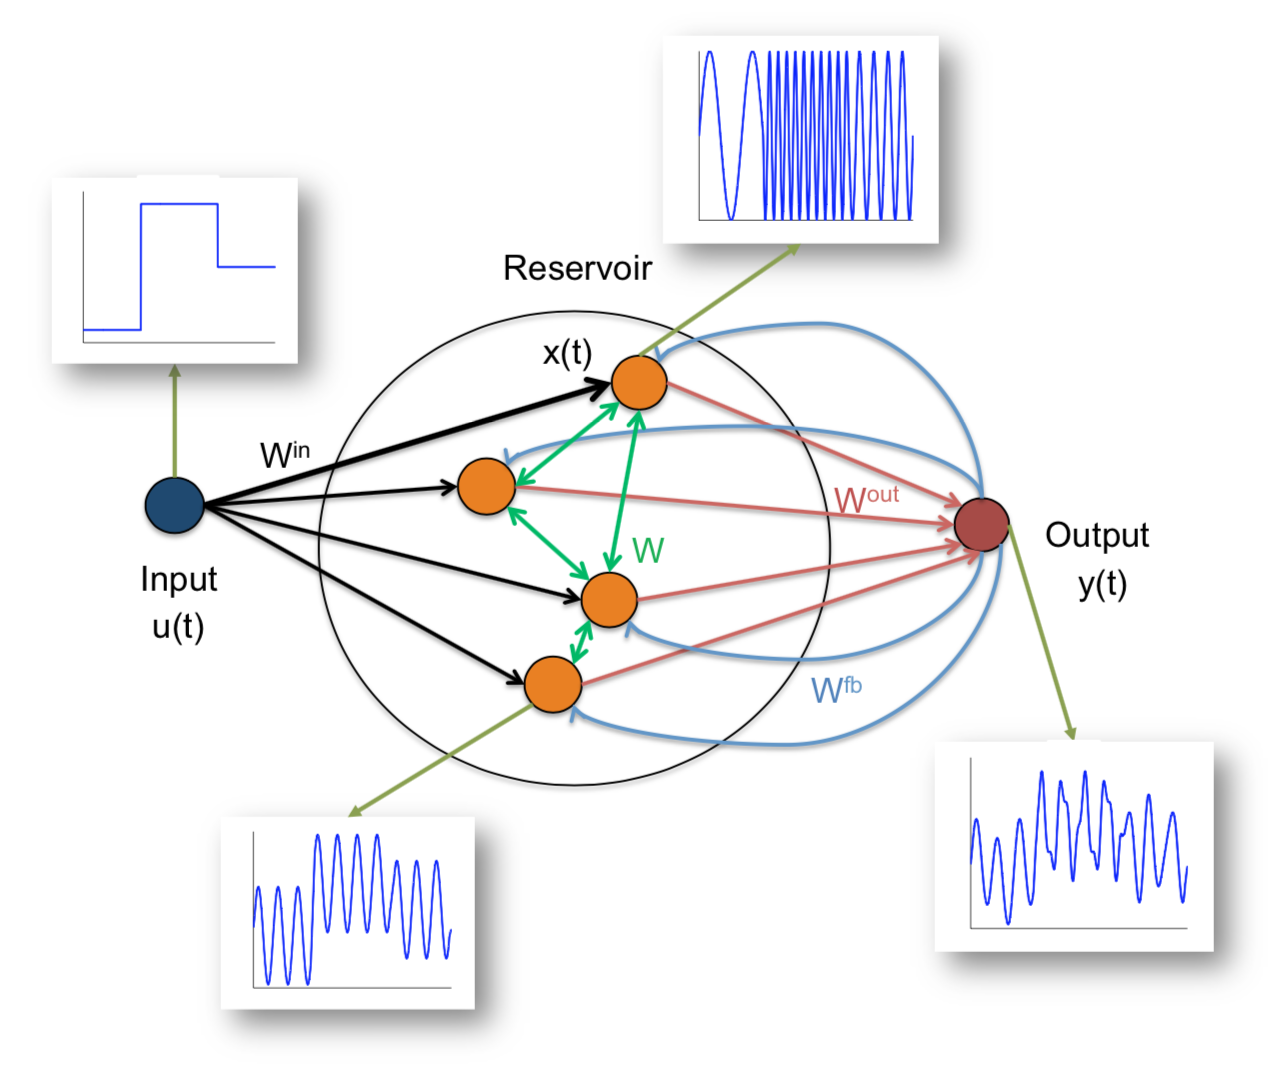
\includegraphics[width=\textwidth]{rc_principle.png}
		\caption{\cite{financialTimeSeries}}
	\end{figure}
	
	\end{column}%
	\end{columns}
\end{frame}

\begin{frame}{Simulation - NARMA 10}
	\begin{columns} % align columns
	\begin{column}{.33\textwidth}
	
		\begin{itemize}
			\item Nonlinear AutoRegressive Moving Average
			\item 50 neurons
			\item Washout : 300
			\item Learning : 3000
			\item Testing : 6000
			\item NMSE = 0.1439
		\end{itemize}
		
	\end{column}%
	\hfill%
	\begin{column}{.63\textwidth}
		\begin{figure}
		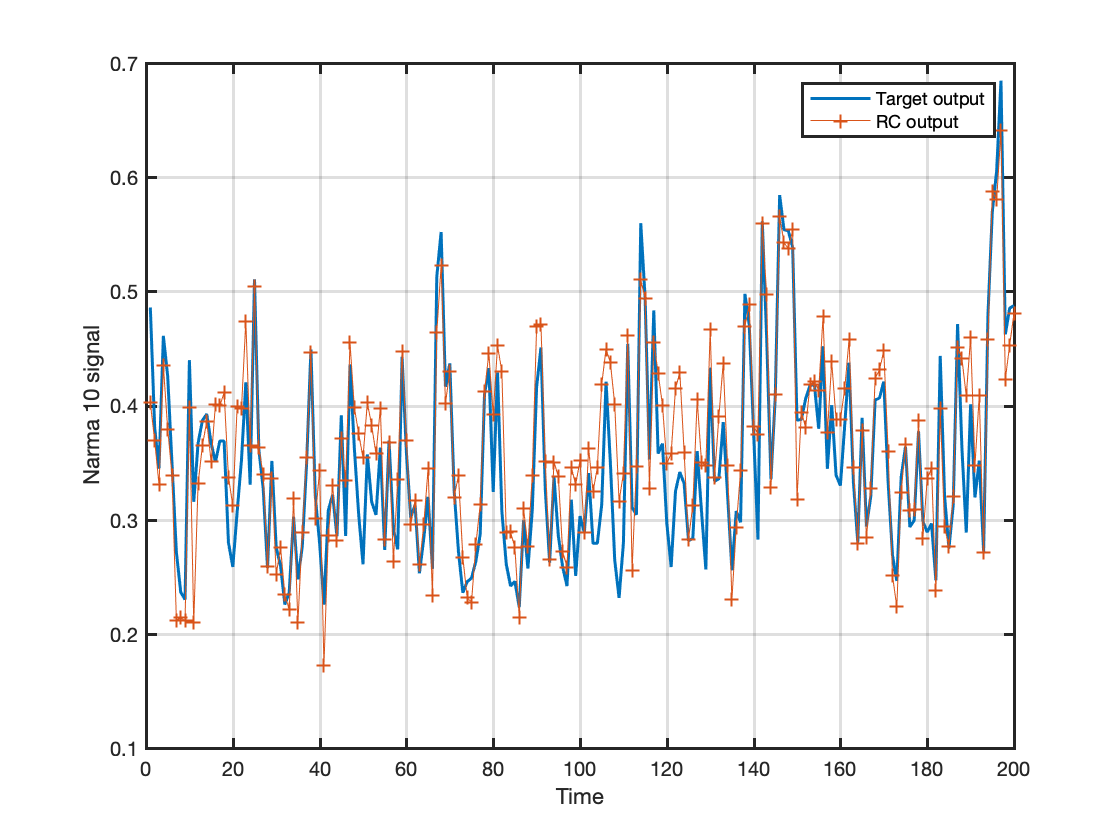
\includegraphics[width=\textwidth]{narma10.png}
	\end{figure}
	
	\end{column}%
	\end{columns}



\end{frame}

\begin{frame}{Simulation - Nonlinear Channel Equalisation}

	\begin{columns} % align columns
	\begin{column}{.33\textwidth}
	
		\begin{itemize}
			\item 50 neurons
			\item SNR = 32 dB
			\item Washout : 300
			\item Learning : 3000
			\item Testing : 6000
			\item SER= $3.33 \cdot 10^{-4}$
		\end{itemize}
		
	\end{column}%
	\hfill%
	\begin{column}{.63\textwidth}
	\begin{figure}
		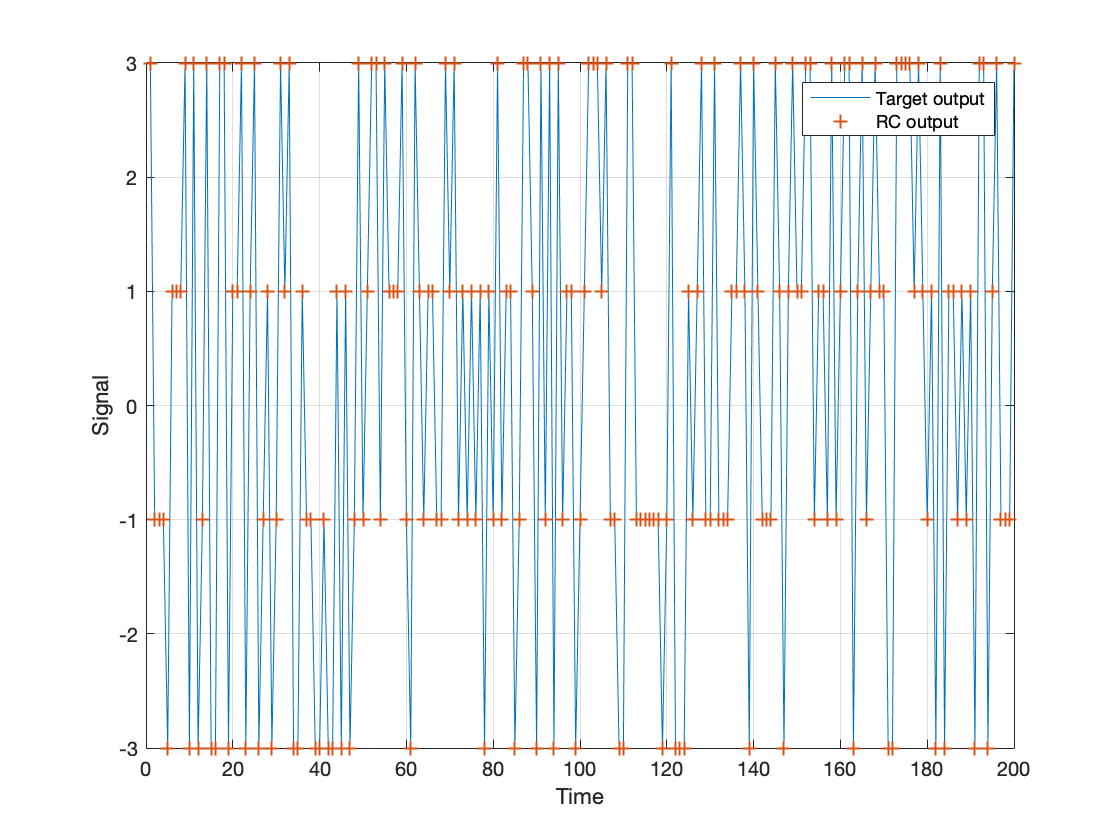
\includegraphics[width=\textwidth]{nonlinear_ch.png}
	\end{figure}

	\end{column}%
	\end{columns}
	
\end{frame}
